\documentclass[11pt,conference]{IEEEtran}

\usepackage{cite}
\usepackage{url}
\usepackage{mathtools}
\usepackage{tikz}

\usetikzlibrary{matrix, fit}
\usetikzlibrary{backgrounds}
\usetikzlibrary{positioning}
\usetikzlibrary{cd}

\def\BibTeX{{\rm B\kern-.05em{\sc i\kern-.025em b}\kern-.08em
    T\kern-.1667em\lower.7ex\hbox{E}\kern-.125emX}}

% a quote environment with less left indent and no right indent
\newenvironment{myquote}{\list{}{\leftmargin=12pt\rightmargin=0pt}\item[]}{\endlist}

% "tabs" for indenting Alloy statements
\def\TA{\makebox[12pt]{}}
\def\TB{\makebox[24pt]{}}
\def\TC{\makebox[36pt]{}}
\def\TD{\makebox[48pt]{}}
\def\TE{\makebox[60pt]{}}

% boldface for Alloy keywords
\def\Bopen{\textbf{open} }
\def\Bas{\textbf{as} }
\def\Bsig{\textbf{sig} }
\def\Babstract{\textbf{abstract} }
\def\Bextends{\textbf{extends} }
\def\Bset{\textbf{set} }
\def\Bpred{\textbf{pred} }
\def\Bfact{\textbf{fact} }
\def\Bfun{\textbf{fun} }
\def\Bassert{\textbf{assert} }
\def\Ball{\textbf{all} }
\def\Bsome{\textbf{some} }
\def\Bone{\textbf{one} }
\def\Belse{\textbf{else} }
\def\Bin{\textbf{in} }
\def\Band{\textbf{and} }
\def\Bor{\textbf{or} }
\def\Bnot{\textbf{not} }
\def\Bno{\textbf{no} }
\def\Bimplies{$\Rightarrow$ }
\def\Biff{\textbf{iff} }
\def\Blet{\textbf{let} }
\def\Bseq{\textbf{seq} }
\def\Bint{\textbf{Int}}
\def\Buniv{\textbf{univ}}
\def\Blone{\textbf{lone} }

\begin{document}

\title{Sparse}
% \author{
%   \IEEEauthorblockN{Tristan Dyer}
%   \and
%   \IEEEauthorblockN{John Baugh}
% }

\maketitle

\section{Introduction}

%Computations on sparse matrices are prevalent in scientific and engineering software.  
Sparse matrix data formats are able to compress large matrices with a small number of non-zero elements into a more efficient representation.  
%The development of software that makes use of sparse matrices is a tedious and often error-prone task because of the myriad data formats and complexities involved in tuning the operations on these formats to achieve an efficient implementation.
Scientific and engineering software that make use of sparse matrix formats are often implemented in low-level imperative languages such as C++ and Fortran.  The optimized nature of these software often means that the structural organization of sparse matrix formats and mathematical computations are heavily intertwined.  Additionally, the myriad data formats and complexities involved in tuning the operations on these formats to achieve efficient implementations means that the development of software that makes use of sparse matrices is a tedious and often error-prone task.

Need to add something about how verification of sparse matrix codes is also difficult, and has only really been done by Arnold.  This is one of our major contributions: sparse matrix codes are difficult to verify (see Arnold), and the development of representation invariants for a number of formats can make this easier.  The representation invariants can be directly translated into code, and used during the development and debugging process to verify that operations on matrices never violate the representation invariants (a la Liskov).

A number of approaches have been taken in order to address these issues.  Object-oriented libraries such as PETSc~\cite{petsc2019} and Eigen~\cite{eigenweb2010} provide data abstractions targeted towards specific classes of solvers.  These libraries provide templates that allow developers to assemble sparse matrices without having to address the structural complexities that a specific format may present.  These matrices can then be used in a variety of solvers, given that the format is supported.

Alternatively, there is a body of research that takes the approach of designing and building compilers capable of automatically making decisions about sparse matrix formats and operations.  Some compilers~\cite{bik1995, bik1996} allow developers to work with dense matrices in code, generating a sparse matrix program at compile time.  Others~\cite{kotlyar1997} allow the user to provide the compiler with an abstract description of a sparse format, from which the compiler can make automatic optimizations in code that accesses the sparse data.

We describe an approach that allows developers to reason about the inherent complexities of sparse matrix formats and operations and to determine invariants that can be used to verify implementations.
%Rather than hiding the complexities of sparse matrix formats by providing data abstractions in code or automatic optimizations in compilers, we propose an approach that allows developers to reason about these complexities.  
Elements of this approach include declarative modeling and automatic, push-button analysis using the Alloy Analyzer~\cite{jackson2012}, a lightweight bounded model checking tool.  Characteristics of sparse matrices, with their numerous representations and ...hard-to-get-right-implementation-details... are approached using abstraction based methods~\cite{clarke1994}, including data abstraction~\cite{dingel1995} and predicate abstraction~\cite{graf1997}, data and functional refinement~\cite{woodcock1996}, and other techniques, manually, as part of a modeling process...

The benefits of this approach lie in its generality.  By using Alloy to perform the modeling and analysis, the modeler may choose the programming language that best fits their needs when transitioning from model to implementation.
Can reason about existing software.
Can reason about design of new sparse matrix libraries.
Can reason about compiler design.

\section{Related Work}

\textbf{Verifying sparse matrix code.}  Arnold et al.~\cite{arnold} design a functional language and proof method for the automatic verification of sparse matrix codes.  Their ``little language" (LL) can be used to specify sparse codes as functional programs in which computations are sequences of high-level transformations on lists.  These models are then automatically translated into Isabelle/HOL where they can be verified for full functional correctness.  The authors use this automated proof method to verify a number of sparse matrix formats and their sparse matrix-vector multiplication operations.  Their approach is purely functional, relying on typed $\lambda$-calculus and Isabelle libraries to perform proofs using Isabelle/HOL.  LL, a shallow embedding in Isabelle/HOL, provides simple, composable rules that can be used to fully describe a sparse matrix format, removing the burden of directly writing proofs.  In quantifying rule reuse, the authors find that ``on average, fewer than 19\% of rules used by a particular format are specific to this format, while over 66\% of these rules are used by at least three additional formats, a significant level of reuse.  Even of the rules needed for more complex formats (CSC and JAD), only up to a third are format-specific.''~\cite{arnold}  The method enables a significant amount of rule reuse, but does not entirely prevent one from having to write some amount of $\lambda$-calculus.  Filling in these gaps may prove difficult for those without a strong background in functional programming and theorem proving.  Our approach, on the other hand, may appeal to an audience of scientists and engineers, who are accustomed to working with models anyway, and with the kind of automatic, push-button analysis supported by Alloy, those who develop software can focus on modeling and design instead of theorem proving.

Arnold approach does not support modeling of assembly of sparse matrices.  Relational approach in combination with state change allows us to model the assembly process as well as updates to matrix values.  Relational approach also allows for modeling of format conversions.

\section{Lightweight Formal Methods}

...
An additional aspect of lightweight formal methods is an incremental style of modeling, which tools like Alloy support by offering immediate feedback while models are being constructed: we start with a minimal set of constraints and ``grow'' them via conjunction.

\subsection{Alloy}

The tool used in our approach is Alloy, a declarative modeling language combining first-order logic with relational calculus and associated quantifiers and operators, along with transitive closure.  It offers rich data modeling features based on class-like structures and an automatic form of analysis that is performed within a bounded scope using a SAT solver.  For \emph{simulation}, the analyzer can be directed to look for instances satisfying a property of interest.  For \emph{checking}, it looks for an instance violating an assertion: a counterexample.  The approach is \emph{scope complete} in the sense that all cases are checked within user-specified bounds.  Alloy's logic supports three distinct styles of expression, that of predicate calculus, navigation expressions, and relational calculus.  The language used for modeling is also used for specifying properties of interest and assertions.  Alloy supports expressions with integer values and basic arithmetic operations.

\subsection{Data Abstraction}

Proof obligations: mathematical formula to be proven in order to ensure that a component is correct.

Start example here.

\subsection{Data Refinement}

The process of data refinement involves removing nondeterminism, or uncertainty, from an abstract model~\cite{woodcock1996}.  While an abstract model may omit certain design choices, a refinement can resolve some of these choices, removing uncertainty and approaching the level of a concrete implementation.

\begin{figure}
\begin{tikzpicture}
\begin{tikzcd}[sep=huge]
AS \arrow{r}[description]{AF} & AS' \\
IS \arrow{u}[description]{\alpha} \arrow{r}[description]{IF} & IS' \arrow{u}[description]{\alpha}
\end{tikzcd}
\end{tikzpicture}
\caption{TODO: An abstract state (AS) becomes new abstract state (AS') through an abstract function (AF).  An implemented state (IS) becomes a new implemented state (IS') through an implemented function (IF).  The implemented states are related to the abstract states through the abstraction function $\alpha$.}
\end{figure}

Abstraction function and representation invariant discussion.

Continue example with refinement here.

\section{Sparse Matrix Models}

In this section we introduce some basic modeling elements used throughout the study, and then we describe four models.  First we describe an abstract model of a matrix that does not represent any specific data format, leaving out all implementation details and notions of sparsity. Then we describe three refinements of this model which introduce structure that supports a sparse representation: the DOK format, the ELL format, and the CSR format.  For each matrix representation we model initialization, update, and matrix-vector multiplication.  For each refinement, we provide representation invariants and abstraction functions to show that the refinement is sound.

By design, Alloy provides no means of working with floating point values.  It includes integers, but in a limited scope, and so they are not useful when attempting to work with the complete integer set, as might be the case when considering values that could be stored in a sparse matrix.  This is inconsequential, however, as we only aim to reason about the structural complexities of sparse matrix formats.  Therefore, it is sufficient to create an abstract distinction between zero and non-zero values.  Our models employ a Value signature, representing any numerical value, and a Zero signature, an extension of Value, that represents the value zero.  Depending on the scope, this creates an abstract set of values, shown in \figurename~\ref{fig:values}, that we can use to populate matrices in our models.

\begin{figure}
\begin{displaymath}
Value = \{Zero, Value_0, Value_1, \ldots, Value_n\}
\end{displaymath}
\caption{The set of abstract values.}
\label{fig:values}
\end{figure}

Throughout these models we make use of predicate overloading to define various predicates that can be applied universally.  Overloading is enabled by Alloy's type system and type checker, which allow expressions to share a name as long as there is no ambiguity when resolving types.  For example, the \texttt{rowInRange} and \texttt{colInRange} predicates are used to determine if a row or column index is within the bounds of some matrix.  The predicate definitions for the three sparse matrix types considered in this study are shown in \figurename~\ref{fig:overload}.  The \texttt{rowInRange} predicate evaluates to true if the value \texttt{row} is greater than or equal to zero and less than the number of rows in, for example, the DOK matrix \texttt{d}, false otherwise.  Similarly, the \texttt{colInRange} predicate evaluates to true if the value \texttt{col} is greather than or equal to zero and less than the number of columns in the DOK matrix \texttt{d}.  Additional usage of overloading found in these models includes the representation invariant, which is always named \texttt{repInv}, and the abstraction function, which is always named \texttt{alpha}.

\begin{figure}
\centering
\begin{myquote}\small{\texttt{\\
\Bpred rowInRange[d: DOK, row: Int] \{\ldots\}\\
\Bpred rowInRange[e: ELL, row: Int] \{\ldots\}\\
\Bpred rowInRange[c: CSR, row: Int] \{\ldots\}\\
\Bpred colInRange[d: DOK, col: Int] \{\ldots\}\\
\Bpred colInRange[e: ELL, col: Int] \{\ldots\}\\
\Bpred colInRange[c: CSR, col: Int] \{\ldots\}\\
}}
\end{myquote}
\caption{Predicate overloading of \texttt{rowInRange} and \texttt{colInRange}.}
\label{fig:overload}
\end{figure}

\subsection{Abstract Sparse Matrix}

We begin with an abstract model of a two-dimensional mathematical matrix, sparse or otherwise, defined by the Matrix signature as shown in \figurename~\ref{model:abstract}.  There are three fields defined on the Matrix signature representing (1) the number of rows in the matrix, (2) the number of columns in the matrix, and (3) the values and their locations in the matrix.  This model makes no assumptions about the contents or structure of the matrix, and will be the arbiter of correctness when determining if a refinement is sound.

\begin{figure}
\centering
\begin{myquote}\small{\texttt{\\
\Bsig Matrix \{\\
\TA  nrows, ncols: \Bint,\\
\TA  values: \Bint~$\rightarrow$~\Bint~$\rightarrow$~Value\\
\} \{\\
\TA nrows $\geq$ 0\\
\TA ncols $\geq$ 0\\
\TA \Ball i, j: \Bint~$|$\\
\TB i $\rightarrow$ j \Bin values.univ \Bimplies\\
\TC 0 $\leq$ i \Band i $<$ nrows \Band\\
\TC 0 $\leq$ j \Band j $<$ ncols\\
\TA \Blet nvals = mul[nrows, ncols] $|$\\
\TB \#values = nvals \Band\\
\TB \#values.univ = nvals\\
\}
}}
\end{myquote}
\caption{The abstract matrix model.}
\label{model:abstract}
\end{figure}

The representation invariant is specified as a signature fact so that it is applied to every member of the Matrix signature.  The representation invariant states that (1) the number of rows and columns in a matrix are each greater than or equal to zero, (2) all row, column indices fall within bounds, (3) the total number of values in the matrix is $\texttt{rows}\times\texttt{cols}$, and (4) there is a value at every $\left(i, j\right)$ index pair.

\subsubsection{Matrix Initialization}

\begin{figure}
\centering
\begin{myquote}\small{\texttt{\\
\Bpred init [m: Matrix, rows, cols: Int] \{\\
\TA m.nrows = rows\\
\TA m.ncols = cols\\
\TA \Blet valset = m.values[\Buniv][\Buniv] |\\
\TB valset = Zero \Bor \Bno valset\\
\}
}}
\end{myquote}
\caption{The abstract matrix initialization.}
\label{init:abstract}
\end{figure}

The \texttt{init} predicate shown in \figurename~\ref{init:abstract} is used to initialize an empty matrix.  We consider the initialized state of a matrix to be one in which the number of rows and columns is defined and all values are zero.

\subsubsection{Matrix Update}

\begin{figure}
\centering
\begin{myquote}\small{\texttt{\\
\Bpred update [m, m': Matrix,\\
\TD row, col: \Bint,\\
\TD val: Value] \{\\
\TA m.rows = m'.rows\\
\TA m.cols = m'.cols\\
\TA rowInRange[m, row]\\
\TA colInRange[m, col]\\
\TA \Blet curr = m.values[row][col] |\\
\TB m'.values =\\
\TC m.values\\
\TC - row$\rightarrow$col$\rightarrow$curr\\
\TC + row$\rightarrow$col$\rightarrow$val\\
\}
}}
\end{myquote}
\caption{The abstract matrix update.}
\label{update:abstract}
\end{figure}

The \texttt{update} predicate shown in \figurename~\ref{update:abstract} is used to perform an update.  We consider a matrix update to be a transition in which a single value of a matrix is changed and the matrix does not change size.  For all matrices, this includes four possible transitions: non-zero to non-zero, non-zero to zero, zero to non-zero, and zero to zero, or stutter.

\subsection{DOK Format}

The dictionary of keys (DOK) format uses a dictionary, or associative array, to store key, value pairs.  An associative array is a collection of key, value pairs in which each possible key may appear only once.  Sparse matrices are stored such that pairs of row, column indices are used as keys to reference stored values.  The DOK format is frequently used~\cite{scipy, eigenweb2010} in the assembly of sparse matrices because of the efficient \(\mathcal{O}(1)\) access to individual elements provided by the associative array format.  However, because associative arrays make no guarantees about memory locality, iterating over all values in the matrix can be inefficient.  As a result, it is common to use this format to incrementally assemble the full matrix and convert it to another sparse matrix format that allows for more efficient operations on matrices.

The DOK signature, shown in \figurename~\ref{model:dok}, resembles the Matrix signature.  The \texttt{nrows} field represents the integer number of rows in the matrix and the \texttt{ncols} field represents the integer number of columns in the matrix.  The \texttt{dict} field represents the dictionary of key, value pairs.  It takes the same form as the values field of the Matrix signature, but the \(\Bint \to \Bint\) relation represents integer pairs used as keys in the dictionary.

\begin{figure}
\centering
\begin{myquote}\small{\texttt{\\
\Bsig DOK \{\\
\TA nrows, ncols: \Bint,\\
\TA dict: \Bint~$\rightarrow$~\Bint~$\rightarrow$~Value\\
\}
}}
\end{myquote}
\caption{The DOK Model.}
\label{model:dok}
\end{figure}

\subsubsection{Representation Invariant}

The representation invariant for the DOK format, shown in \figurename~\ref{repinv:dok}, states that (1) there are no zeros stored as values, (2) all row, column indices used as keys fall within the bounds of the matrix, and (3) all row, column indices that fall within the bounds of the matrix may appear at most once as keys in the dictionary.

\begin{figure}
\centering
\begin{myquote}\small{\texttt{\\
\Bpred repInv [d: DOK] \{\\
\TA Zero \Bnot \Bin d.dict[\Buniv][\Buniv]\\
\TA \Ball i, j: \Bint~\{\\
\TB i$\rightarrow$j \Bin d.dict.univ \Bimplies\\
\TC rowInRange[d, i] \Band\\
\TC colInRange[d, j]\\
\TA \}\\
\TA \Ball i, j: \Bint~\{\\
\TB rowInRange[d, i] \Band\\
\TB colInRange[d, j] \Bimplies\\
\TC \Blone v: Value | i$\rightarrow$j$\rightarrow$v \Bin d.dict\\
\TA \}\\
\}\\
}}
\end{myquote}
\caption{The DOK representation invariant.}
\label{repinv:dok}
\end{figure}

\subsubsection{Abstraction Function}

The abstraction function provides a mapping from the DOK representation of a matrix to our abstract representation of a matrix.  The \texttt{alpha} predicate, shown in \figurename~\ref{alpha:dok}, states that the DOK matrix $d$ is a refinement of Matrix $m$ if (1) $d$ has the same number of rows and columns as $m$, (2) all row, column index pairs that map to a value in the $d$ dictionary map to the same value at the same location in $m$, and (3) all in-range row, column pairs \emph{not} used as keys in the $d$ dictionary map to zeros in $m$.

\begin{figure}
\centering
\begin{myquote}\small{\texttt{\\
\Bpred alpha [d: DOK, m: Matrix] \{\\
\TA m.rows = d.rows\\
\TA m.cols = d.cols\\
\TA \Ball i, j: \Bint, v: Value |\\
\TB i$\rightarrow$j$\rightarrow$v \Bin d.dict \Bimplies\\
\TC i$\rightarrow$j$\rightarrow$v \Bin m.values\\
\TA \Ball i, j: Int |\\
\TB rowInRange[d, i] and\\
\TB colInRange[d, j] and\\
\TB i$\rightarrow$j not in d.dict.\Buniv~\Bimplies\\
\TC i$\rightarrow$j$\rightarrow$Zero \Bin m.values\\
\}
}}
\end{myquote}
\caption{The DOK abstraction function}
\label{alpha:dok}
\end{figure}

\subsubsection{Matrix Initialization}

Initialization of the DOK matrix, shown in \figurename~\ref{init:dok}, requires setting the size of the matrix and creating an empty dictionary.  Because the abstraction function maps indices that aren't included as keys to zero, an empty dictionary represents a matrix in which all values are zero.

\begin{figure}
\centering
\begin{myquote}\small{\texttt{\\
\Bpred init [d: DOK, rows, cols: Int] \{\\
\TA d.nrows = rows\\
\TA d.ncols = cols\\
\TA \Bno d.dict\\
\}
}}
\end{myquote}
\caption{The DOK initialization predicate.}
\label{init:dok}
\end{figure}

\subsubsection{Matrix Update}

\begin{figure}
\centering
% \begin{myquote}\small{\texttt{\\
% \Bpred ZtoZ[d, d': DOK,\\
% \TE curr, val: Value] \{\\
% \TA \Bno curr\\
% \TA val = Zero\\
% \TA d'.dict = d.dict\\
% \}
% }}
% \end{myquote}

% \begin{myquote}\small{\texttt{\\
% \Bpred ZtoNZ[d, d': DOK,\\
% \TE row, col: \Bint,\\
% \TE curr, val: Value] \{\\
% \TA \Bno curr\\
% \TA val != Zero\\
% \TA d'.dict = d.dict + row$\rightarrow$col$\rightarrow$val)\\
% \}
% }}
% \end{myquote}

% \begin{myquote}\small{\texttt{\\
% \Bpred NZtoZ[d, d': DOK,\\
% \TE row, col: \Bint,\\
% \TE curr, val: Value] \{\\
% \TA val = Zero\\
% \TA d'.dict = d.dict - row$\rightarrow$col$\rightarrow$curr\\
% \}
% }}
% \end{myquote}

% \begin{myquote}\small{\texttt{\\
% \Bpred NZtoNZ[d, d': DOK,\\
% \TE row, col: \Bint,\\
% \TE curr, val: Value] \{\\
% \TA val != Zero\\
% \TA d'.dict = d.dict\\
% \TB - row$\rightarrow$col$\rightarrow$curr\\
% \TB + row$\rightarrow$col$\rightarrow$val)\\
% \}
% }}
% \end{myquote}

\begin{myquote}\small{\texttt{\\
\Bpred update [d, d': DOK,\\
\TD row, col: \Bint,\\
\TD val: Value] \{\\
\TA d.rows = d'.rows\\
\TA d.cols = d'.cols\\
\TA rowInRange[d, row]\\
\TA colInRange[d, col]\\
\TA \Blet curr = d.dict[row][col] \{\\
\TB ZtoZ[d, d', curr, val] \Bor\\
\TB ZtoNZ[d, d', row, col, curr, val] \Bor\\
\TB NZtoZ[d, d', row, col, curr, val] \Bor\\
\TB NZtoNZ[d, d', row, col, curr, val]\\
% \TB (\Bno curr \Band val != Zero \Band\\
% \TC d'.dict = d.dict + row$\rightarrow$col$\rightarrow$val)\\
% \TB \Bor\\
% \TB (\Bno curr \Band val = Zero \Band\\
% \TC d'.dict = d.dict)\\
% \TB \Bor\\
% \TB (val != Zero \Band d'.dict = d.dict\\
% \TC - row$\rightarrow$col$\rightarrow$curr\\
% \TC + row$\rightarrow$col$\rightarrow$val)\\
% \TB \Bor\\
% \TB (val = Zero \Band d'.dict = d.dict\\
% \TC - row$\rightarrow$col$\rightarrow$curr)\\
\TA\}\\
\}
}}
\end{myquote}
\caption{The DOK update predicate.}
\label{update:dok}
\end{figure}

\subsubsection{SpMV}

\subsection{ELL Format}

ELL, coming soon.

\subsection{CSR Format}

The Compressed Sparse Row (CSR) format, shown in \figurename~\ref{image:csr}, uses three arrays to store a sparse matrix, one for values and two for integers.  The value array contains non-zero values of the matrix ordered as they are traversed in a row-wise fashion.  Column indices of each value are stored in a separate array, while a third array stores the location in the values array that starts each row.  We adopt the convention that the values array is named $\mathrm{A}$, the column array is named $\mathrm{JA}$, and the row index array is name $\mathrm{IA}$.

\begin{figure}
\centering
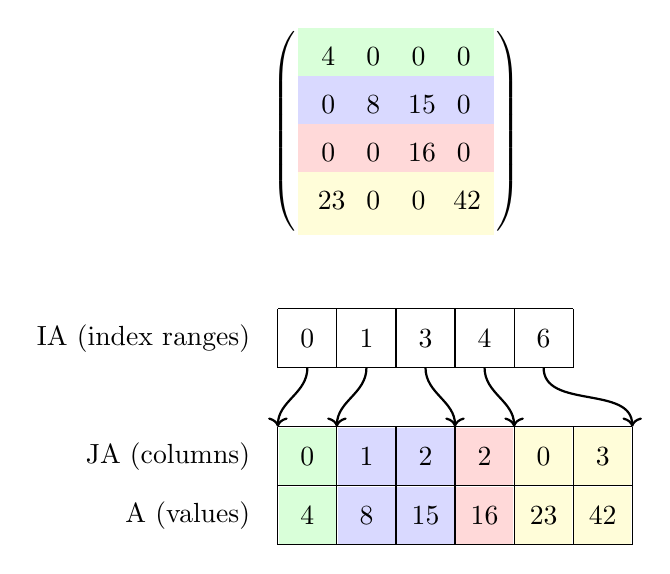
\begin{tikzpicture}

\begin{scope}[every node/.style={minimum size=0.75cm-2*\pgflinewidth, outer sep=0pt},scale=0.75]
\draw (0,0) grid +(5,1);
\node (ia) at (0.5, 0.5) {0};
\node at (1.5, 0.5) {1};
\node at (2.5, 0.5) {3};
\node at (3.5, 0.5) {4};
\node at (4.5, 0.5) {6};

\draw(0,-1) grid +(6,-2);

\node[fill=green!15] (ja) at (0.5, -1.5) {0};
\node[fill=blue!15] at (1.5, -1.5) {1};
\node[fill=blue!15] at (2.5, -1.5) {2};
\node[fill=red!15] at (3.5, -1.5) {2};
\node[fill=yellow!15] at (4.5, -1.5) {0};
\node[fill=yellow!15] at (5.5, -1.5) {3};

\node[fill=green!15] (a) at (0.5, -2.5) {4};
\node[fill=blue!15] at (1.5, -2.5) {8};
\node[fill=blue!15] at (2.5, -2.5) {15};
\node[fill=red!15] at (3.5, -2.5) {16};
\node[fill=yellow!15] at (4.5, -2.5) {23};
\node[fill=yellow!15] at (5.5, -2.5) {42};

\draw [thick,->] (0.5,0) to[out=-90, in=90] (0, -1.0);
\draw [thick,->] (1.5,0) to[out=-90, in=90] (1, -1.0);
\draw [thick,->] (2.5,0) to[out=-90, in=90] (3, -1.0);
\draw [thick,->] (3.5,0) to[out=-90, in=90] (4, -1.0);
\draw [thick,->] (4.5,0) to[out=-90, in=90] (6, -1.0);

\node[left = 0.25cm of ia] {$\mathrm{IA}$ (index ranges)};
\node[left = 0.25cm of ja] {$\mathrm{JA}$ (columns)};
\node[left = 0.25cm of a]  {$\mathrm{A}$ (values)};
\end{scope}

\matrix[
    matrix of math nodes,
    row sep=.5ex,
    column sep=.5ex,
    left delimiter=(,right delimiter=),
    nodes={text width=.75em, text height=1.5ex, text depth=.5ex, align=center}
    ] (m) at (1.5, 3)
    {
    4 & 0 & 0 & 0 \\
    0 & 8 & 15 & 0 \\
    0 & 0 & 16 & 0 \\
    23 & 0 & 0 & 42 \\
    };

\begin{scope}[on background layer]
    \node[fit=(m-1-1)(m-1-4), draw=green!15, fill=green!15] {};
    \node[fit=(m-2-1)(m-2-4), draw=blue!15, fill=blue!15] {};
    \node[fit=(m-3-1)(m-3-4), draw=red!15, fill=red!15] {};
    \node[fit=(m-4-1)(m-4-4), draw=yellow!15, fill=yellow!15] {};
\end{scope} 

\end{tikzpicture}
\caption{The CSR format.}
\label{image:csr}
\end{figure}

The CSR format, making no assumptions about the sparsity structure of the matrix, is a general format capable of compressing any sparse matrix.  The storage savings for this approach is significant, requiring $2nnz+n+1$ storage locations\footnote{where $n$ is the number of rows, $m$ is the number of columns, and $nnz$ is the number of non-zero values} rather than $n \times m$.  Memory locality is improved for row access over the DOK format, but the indirect addressing steps can have an impact on performance~\cite{bai}.

\begin{figure}
\centering
\begin{myquote}\small{\texttt{\\
\Bsig CSR \{\\
\TA nrows, ncols: \Bint,\\
\TA A: \Bseq Value,\\
\TA IA, JA: \Bseq \Bint,\\
\}
}}
\end{myquote}
\caption{The CSR model.}
\label{model:csr}
\end{figure}

Need to describe the ``get'' predicate and why it is needed.

\begin{figure}
\centering
\begin{myquote}\small{\texttt{\\
\Bfun get [c: CSR, row, col: Int]: Value \{
\TA let a = c.IA[row],\\
\TC b = c.IA[add[row, 1]] \{\\
\TB (\Bno a \Bor \Bno b \Bor a = b) \Bimplies Zero\\
\TB \Belse \{\\
\TC \Blet j = c.JA.subseq[a, sub[b, 1]],\\
\TE v = c.A.subseq[a, sub[b, 1]],\\
\TE i = j.idxOf[col] \{\\
\TD \Bno i \Bimplies Zero \Belse v[i]\\
\TC \}\\
\TB \}\\
\TA \}\\
\}
}}
\end{myquote}
\caption{The get function used in the CSR model.}
\label{get:csr}
\end{figure}

The abstraction function:

\begin{figure}
\centering
\begin{myquote}\small{\texttt{\\
\Bpred alpha [c: CSR, m: Matrix] \{\\
\TA m.nrows = c.nrows\\
\TA m.ncols = c.ncols\\
\TA \Ball i, j: \Bint~|\\
\TB rowInRange[c, i] \Band\\
\TB colInRange[c, j] \Bimplies\\
\TC m.values[i][j] = get[c, i, j]\\
\}
}}
\end{myquote}
\caption{The CSR abstraction function.}
\label{alpha:csr}
\end{figure}

The representation invariant:

\begin{figure}
\centering
\begin{myquote}\small{\texttt{\\
\Bpred repInv [c: CSR] \{\\
\TA Zero \Bnot \Bin y.A.elems\\
\TA \Ball i: y.IA.rest.elems |\\
\TB gte[i, 0] \Band\\
\TB lte[i, mul[y.rows, y.cols]]\\
\TA \Ball j: y.JA.elems |\\
\TB gte[j, 0] \Band\\
\TB lt[j, y.cols]\\
\TA y.IA[0] = 0\\
\TA y.IA.last = \#y.A\\
\TA \#y.IA $>$ 1 \Bimplies\\
\TC gt[y.IA.last, y.IA.butlast.last]\\
\TA \#y.A = \#y.JA\\
\TA lte[\#y.A, mul[y.rows, y.cols]]\\
\TA lte[\#y.IA, add[y.rows, 1]]\\
\TA \Ball i: y.IA.inds |\\
\TB i > 0 \Bimplies\\
\TC \Blet a = y.IA[sub[i, 1]],\\
\TC       b = y.IA[i],\\
\TC       n = sub[b, a] \{\\
\TD   b $\geq$ a\\
\TD   n $\leq$ y.cols\\
\TD   n = \#y.JA.subseq[a, sub[b, 1]].elems\\
\TC \}\\
\}
}}
\end{myquote}

% \begin{itemize}
%   \item The integer value \(nrows \geq 0\)
%   \item The integer value \(ncols \geq 0\)
% 	\item There are no zeros stored as values
% 	\item All values in IA \(\leq nrows \times ncols\)
% 	\item All values in JA \(< ncols\)
% 	\item The first value in IA is zero
% 	\item The last value in IA is the length of A
% 	\item The last value of IA is not repeated
% 	\item A and JA are the same length
% 	\item The max length of A is \(nrows \times ncols\)
% 	\item The max length of IA is \(nrows + 1\)
% 	\item The values in IA are monotonically increasing
% 	\item The difference between any two consecutive values in IA must be \(\leq ncols\)
% 	\item Values in JA must be unique per row
% \end{itemize}
\caption{The CSR representation invariant.}
\label{repinv:csr}
\end{figure}

\section{Sparse Matrix Code}

Show how representation invariants can be used in code.

\bibliographystyle{IEEEtran}
\bibliography{IEEEabrv,sparse,mybib}

\end{document}
